% ============================================================
% Chapter 05 — 频域分析
% ============================================================

\chapter{频域分析}

\intro{频域分析法是控制理论中最重要的分析方法之一。它通过研究系统在不同频率正弦输入下的稳态响应，揭示系统的动态特性。频域法不仅能用于稳定性分析，还可直接用于系统设计和校正，是经典控制理论的核心工具。}

% ============================================================
\section{频率特性的基本概念}
% ============================================================

\subsection{频率特性的定义}

设线性定常系统的传递函数为 $G(s)$，当输入为正弦信号 $r(t) = A_r \sin(\omega t)$ 时，系统稳态输出为同频率的正弦信号：
\[
y_{\text{ss}}(t) = A_r |G(j\omega)| \sin(\omega t + \angle G(j\omega))
\]

\begin{mydefinition}{频率特性}
传递函数 $G(s)$ 中令 $s = j\omega$，得到的复变函数 $G(j\omega)$ 称为系统的\textbf{频率特性}。

\[
G(j\omega) = |G(j\omega)| e^{j\angle G(j\omega)} = A(\omega) e^{j\varphi(\omega)}
\]

其中 $A(\omega)=|G(j\omega)|$ 为\textbf{幅频特性}，$\varphi(\omega)=\angle G(j\omega)$ 为\textbf{相频特性}。
\end{mydefinition}

\begin{myTheorem}{频率特性的物理意义}
频率特性 $G(j\omega)$ 的模 $|G(j\omega)|$ 等于稳态输出与输入的幅值之比，辐角 $\angle G(j\omega)$ 等于稳态输出与输入的相位差。
\end{myTheorem}

\begin{proof}
设系统输入 $r(t) = A_r \sin(\omega t)$，其 Laplace 变换为
\[
R(s) = \frac{A_r \omega}{s^2 + \omega^2}
\]
输出 $Y(s) = G(s)R(s)$，展开为部分分式后取 Laplace 反变换。当 $t \to \infty$ 时，暂态分量趋于零，稳态分量为
\[
y_{\text{ss}}(t) = A_r |G(j\omega)| \sin\bigl(\omega t + \angle G(j\omega)\bigr)
\]
证毕。
\end{proof}

\subsection{频率特性的几何表示}

频率特性可以在复平面上用向量表示。对每一频率 $\omega$，$G(j\omega)$ 对应复平面上的一个点。当 $\omega$ 从 $0$ 变化到 $\infty$ 时，这些点的轨迹构成\textbf{幅相特性曲线}（Nyquist 图）。

\begin{mydefinition}{频率特性的三种表示}
\begin{itemize}
    \item \textbf{幅相频率特性}（Nyquist 图）：以 $\omega$ 为参变量，在复平面上绘制 $\Re[G(j\omega)]$ 和 $\Im[G(j\omega)]$ 的关系。
    \item \textbf{对数频率特性}（Bode 图）：包含对数幅频特性 $L(\omega) = 20\lg |G(j\omega)|$（单位：dB）和对数相频特性 $\varphi(\omega)$（单位：度或弧度），横坐标均为 $\omega$ 的对数分度。
    \item \textbf{对数幅相特性}（Nichols 图）：以 $\varphi(\omega)$ 为横坐标，$L(\omega)$ 为纵坐标，$\omega$ 为参变量。
\end{itemize}
\end{mydefinition}

\begin{example}
考虑一阶惯性环节 $G(s) = \frac{1}{Ts + 1}$，其频率特性为
\[
G(j\omega) = \frac{1}{1 + j\omega T} = \frac{1}{\sqrt{1 + \omega^2 T^2}} e^{-j\arctan(\omega T)}
\]
幅频：$A(\omega) = 1/\sqrt{1 + \omega^2 T^2}$，相频：$\varphi(\omega) = -\arctan(\omega T)$。
当 $\omega = 0$ 时，$A=1$，$\varphi = 0^{\circ}$；
当 $\omega = 1/T$（截止频率）时，$A = 1/\sqrt{2} \approx 0.707$，$\varphi = -45^{\circ}$；
当 $\omega \to \infty$ 时，$A \to 0$，$\varphi \to -90^{\circ}$。
\end{example}

% ============================================================
\section{典型环节的频率特性}
% ============================================================

自动控制系统通常由若干典型环节构成。掌握各典型环节的频率特性是频域分析的基础。

\subsection{比例环节}

传递函数 $G(s) = K$，频率特性 $G(j\omega) = K$。

幅频：$A(\omega) = K$，对数幅频：$L(\omega) = 20\lg K$。
相频：$\varphi(\omega) = 0^{\circ}$。

Nyquist 图为实轴上的一点 $(K, 0)$。Bode 图中幅频为平行于横轴的直线，相频为零度线。

\subsection{积分环节}

传递函数 $G(s) = 1/s$，频率特性 $G(j\omega) = 1/(j\omega) = -j/\omega$。

幅频：$A(\omega) = 1/\omega$，$L(\omega) = -20\lg \omega$（斜率为 $-20$ dB/dec 的直线）。
相频：$\varphi(\omega) = -90^{\circ}$。

Nyquist 图为整个负虚轴。

\subsection{微分环节}

传递函数 $G(s) = s$，频率特性 $G(j\omega) = j\omega$。

$L(\omega) = 20\lg \omega$（$+20$ dB/dec），$\varphi(\omega) = +90^{\circ}$。

Nyquist 图为整个正虚轴。

\subsection{惯性环节}

传递函数 $G(s) = 1/(Ts + 1)$，频率特性
\[
G(j\omega) = \frac{1}{1 + j\omega T} = \frac{1}{1 + \omega^2 T^2} - j\frac{\omega T}{1 + \omega^2 T^2}
\]

\begin{myformula}
L(\omega) = -20\lg\sqrt{1 + \omega^2 T^2},\quad
\varphi(\omega) = -\arctan(\omega T)
\end{myformula}

绘制 Bode 图的渐近线：
\begin{itemize}
    \item 低频段 ($\omega \ll 1/T$)：$L(\omega) \approx 0$ dB，$\varphi(\omega) \approx 0^{\circ}$
    \item 高频段 ($\omega \gg 1/T$)：$L(\omega) \approx -20\lg(\omega T)$，斜率 $-20$ dB/dec，$\varphi(\omega) \approx -90^{\circ}$
    \item 交接频率 $\omega = 1/T$ 处，精确值为 $L = -3$ dB，$\varphi = -45^{\circ}$
\end{itemize}

Nyquist 图为以 $(1/2, 0)$ 为圆心、半径为 $1/2$ 的半圆。

\subsection{振荡环节}

传递函数 $G(s) = \frac{\omega_n^2}{s^2 + 2\zeta\omega_n s + \omega_n^2}$，频率特性
\[
G(j\omega) = \frac{\omega_n^2}{(j\omega)^2 + 2\zeta\omega_n(j\omega) + \omega_n^2} = \frac{1}{\bigl(1 - \frac{\omega^2}{\omega_n^2}\bigr) + j2\zeta\frac{\omega}{\omega_n}}
\]

\begin{myformula}
A(\omega) = \frac{1}{\sqrt{\bigl(1 - \frac{\omega^2}{\omega_n^2}\bigr)^2 + \bigl(2\zeta\frac{\omega}{\omega_n}\bigr)^2}},\quad
\varphi(\omega) = -\arctan\frac{2\zeta\frac{\omega}{\omega_n}}{1 - \frac{\omega^2}{\omega_n^2}}
\end{myformula}

当阻尼比 $\zeta < \sqrt{2}/2 \approx 0.707$ 时，$A(\omega)$ 出现峰值：
\[
M_r = \frac{1}{2\zeta\sqrt{1-\zeta^2}},\quad \omega_r = \omega_n\sqrt{1-2\zeta^2}
\]

Bode 图渐近线：
\begin{itemize}
    \item 低频段 ($\omega \ll \omega_n$)：$L(\omega) \approx 0$ dB
    \item 高频段 ($\omega \gg \omega_n$)：$L(\omega) \approx -40\lg(\omega/\omega_n)$，斜率 $-40$ dB/dec
    \item 交接频率 $\omega_n$ 附近可能出现谐振峰
\end{itemize}

\subsection{滞后环节}

传递函数 $G(s) = e^{-\tau s}$，频率特性 $G(j\omega) = e^{-j\omega\tau}$。

$A(\omega) = 1$，$L(\omega) = 0$ dB，$\varphi(\omega) = -\omega\tau$（随频率线性下降）。

滞后环节不改变幅频特性，仅引入相位滞后，对系统稳定性有不利影响。

\subsection{一阶微分环节}

传递函数 $G(s) = Ts + 1$，频率特性 $G(j\omega) = 1 + j\omega T$。

$L(\omega) = 20\lg\sqrt{1 + \omega^2 T^2}$，高频斜率 $+20$ dB/dec。
$\varphi(\omega) = \arctan(\omega T)$，高频趋近 $+90^{\circ}$。

\begin{myTheorem}{频域特性叠加原理}
设开环系统由若干典型环节串联而成：
\[
G(s) = G_1(s)G_2(s)\cdots G_n(s)
\]
则开环对数幅频和相频特性分别为各环节对数幅频和相频特性的代数和：
\[
L(\omega) = \sum_{i=1}^{n} L_i(\omega),\quad
\varphi(\omega) = \sum_{i=1}^{n} \varphi_i(\omega)
\]
\end{myTheorem}

此叠加性质是 Bode 图在系统分析和设计中被广泛应用的重要原因。

% ============================================================
\section{Bode 图}
% ============================================================

\subsection{对数频率特性的坐标}

Bode 图由两幅图组成：
\begin{itemize}
    \item \textbf{对数幅频特性图}：纵坐标 $L(\omega) = 20\lg|G(j\omega)|$（单位：dB），横坐标按 $\lg\omega$ 分度，标注 $\omega$ 值。
    \item \textbf{对数相频特性图}：纵坐标为 $\varphi(\omega)$（单位：度或弧度），横坐标同样为 $\lg\omega$。
\end{itemize}

频率轴采用对数分度的优点：扩展了低频段，压缩了高频段，能在同一图上表示很宽的频率范围。十倍频程（decade）表示频率增加10倍的区间，二倍频程（octave）表示频率增加1倍的区间。

\begin{myalgorithm}{Bode 图渐近线绘制步骤}
\begin{enumerate}
    \item 将开环传递函数化为典型环节乘积的标准形式，确定各交接频率。
    \item 确定低频段渐近线：在 $\omega < \omega_{\min}$（最小交接频率）处，根据积分环节个数 $\nu$，低频渐近线斜率为 $-20\nu$ dB/dec，过点 $(1, 20\lg K)$。
    \item 在各交接频率处改变斜率：惯性环节加 $-20$ dB/dec，一阶微分加 $+20$ dB/dec，振荡环节加 $-40$ dB/dec。
    \item 在各交接频率处对相频进行修正。
    \item 必要时在交接频率附近对渐近线进行修正（惯性/微分环节修正 $\pm3$ dB，振荡环节按 $\zeta$ 查表修正）。
\end{enumerate}
\end{myalgorithm}

\subsection{系统辨识中的 Bode 图应用}

Bode 图可以用于系统辨识，即通过实验测量的频率响应数据来确定系统的传递函数。基本步骤为：

\begin{enumerate}
    \item 对系统施加不同频率的正弦信号，测量稳态输出的幅值比和相位差。
    \item 在对数坐标纸上绘制实验 Bode 图。
    \item 用斜率为 $\pm20n$ dB/dec ($n$ 为整数) 的渐近线逼近实验幅频曲线。
    \item 根据渐近线的交接频率和斜率变化确定各典型环节参数。
    \item 写出系统的近似传递函数。
\end{enumerate}

\begin{remark}
由最小相位系统的幅频特性可以唯一确定其相频特性和传递函数（Bode 定理），因此实际系统辨识时往往只测量幅频特性即可。
\end{remark}

% --- Bode 图 TikZ ---
\begin{figure}[H]
\centering
\begin{tikzpicture}[
    ctrlBodeXScale/.style={},
    ctrlBodeMagStyle/.style={blue, thick},
    ctrlBodePhaseStyle/.style={red, thick},
    ctrlBodeAsymStyle/.style={blue, dashed, thin},
    ctrlBodeGridStyle/.style={gray!50, very thin},
    >=stealth
]
    % 坐标轴参数
    \def\xmin{-1}\def\xmax{2.5}
    \def\ymagmin{-60}\def\ymagmax{40}
    \def\yphimin{-180}\def\yphimax{0}

    % --- 幅频图 ---
    \begin{scope}
        % 网格
        \foreach \x in {-1,-0.5,...,2.5}
            \draw[ctrlBodeGridStyle] (\x,\ymagmin) -- (\x,\ymagmax);
        \foreach \y in {-60,-40,...,40}
            \draw[ctrlBodeGridStyle] (\xmin,\y) -- (\xmax,\y);

        % 坐标轴
        \draw[->] (\xmin,0) -- (\xmax+0.2,0) node[right] {$\lg\omega$};
        \draw[->] (0,\ymagmin) -- (0,\ymagmax+2) node[above] {$L(\omega)$ (dB)};

        % 渐近线 — 二阶系统示例：$\omega_n=1$, $\zeta=0.3$
        \draw[ctrlBodeAsymStyle] (-1,0) -- (0,0);  % 低频 0dB
        \draw[ctrlBodeAsymStyle] (0,0) -- (2.5,-100); % 高频 -40dB/dec

        % 精确曲线
        \pgfkeys{/pgf/fpu=true,/pgf/fpu/output format=fixed}
        \draw[ctrlBodeMagStyle, domain=-1:1.5, samples=100, smooth]
            plot (\x, {20*log10(1/sqrt((1-10^(2*\x))^2 + (0.6*10^\x)^2))});
        \pgfkeys{/pgf/fpu=false}

        % 标注
        \node[below] at (0,0) {$\omega_n$};
        \draw[dotted] (0,0) -- (0,\ymagmin);
        \node[blue] at (1.8,10) {精确曲线};
        \node[blue!60] at (1.8,5) {渐近线};
    \end{scope}

    % --- 相频图 ---
    \begin{scope}[yshift=-7cm]
        % 网格
        \foreach \x in {-1,-0.5,...,2.5}
            \draw[ctrlBodeGridStyle] (\x,\yphimin) -- (\x,\yphimax);
        \foreach \y in {-180,-135,...,0}
            \draw[ctrlBodeGridStyle] (\xmin,\y) -- (\xmax,\y);

        % 坐标轴
        \draw[->] (\xmin,0) -- (\xmax+0.2,0) node[right] {$\lg\omega$};
        \draw[->] (0,\yphimin) -- (0,\yphimax+5) node[above] {$\varphi(\omega)$ ($^{\circ}$)};

        % 相频精确曲线
        \pgfkeys{/pgf/fpu=true,/pgf/fpu/output format=fixed}
        \draw[ctrlBodePhaseStyle, domain=-1:1.5, samples=100, smooth]
            plot (\x, {-atan2(0.6*10^\x, 1-10^(2*\x))});
        \pgfkeys{/pgf/fpu=false}

        \node[below] at (0,0) {$\omega_n$};
        \draw[dotted] (0,0) -- (0,\yphimin);
        \node at (0,-90) [right] {$-90^{\circ}$};
        \node at (0,-180) [right] {$-180^{\circ}$};
    \end{scope}
\end{tikzpicture}
\caption{典型二阶系统的 Bode 图（渐近线与精确曲线对比）}
\label{fig:bode-second-order}
\end{figure}

% ============================================================
\section{Nyquist 图与稳定性判据}
% ============================================================

\subsection{Nyquist 图的基本概念}

Nyquist 图（幅相频率特性图）是在复平面上以 $\omega$ 从 $0$ 到 $\infty$ 为参变量绘制的 $G(j\omega)$ 轨迹，也称极坐标图。

对于最小相位系统，Nyquist 图的起始点 ($\omega=0$) 和终止点 ($\omega\to\infty$) 分别反映了系统在低频和高频段的特性。

\begin{mydefinition}{围线映射}
设 $F(s)$ 是复变量 $s$ 的有理函数，$\Gamma_s$ 是 $s$ 平面上一条不经过 $F(s)$ 极点的闭合围线。当 $s$ 沿 $\Gamma_s$ 顺时针行走一周时，$F(s)$ 在 $F$ 平面上也形成一条闭合围线 $\Gamma_F$。$\Gamma_F$ 包围原点的圈数等于 $\Gamma_s$ 内 $F(s)$ 的零点数减去极点数。
\end{mydefinition}

\subsection{Cauchy 定理与 Nyquist 稳定判据}

设单位反馈系统的开环传递函数为 $G(s)$，闭环特征方程为 $1 + G(s) = 0$。令
\[
F(s) = 1 + G(s)
\]
则 $F(s)$ 的零点即为闭环极点，$F(s)$ 的极点即为开环极点。

取 Nyquist 围线（包围整个右半 $s$ 平面的大半圆），$F(s)$ 的围线包围原点的圈数为：
\[
N_F = Z - P
\]
其中 $Z$ 为右半平面闭环极点数，$P$ 为右半平面开环极点数。

由于 $F(s) = 1 + G(s)$ 的围线包围原点等价于 $G(s)$ 的围线包围 $(-1, j0)$ 点，故：

\begin{myTheorem}{Nyquist 稳定判据（基本形式）}
设开环系统有 $P$ 个右半平面极点，开环频率特性 $G(j\omega)$ 的 Nyquist 图逆时针包围 $(-1, j0)$ 点的圈数记为 $N$（顺时针为负），则闭环系统稳定的充要条件是
\[
Z = P - N = 0
\]
\end{myTheorem}

\begin{myTheorem}{Nyquist 稳定判据（简化形式）}
若开环系统稳定（$P = 0$），则闭环系统稳定的充要条件是 $G(j\omega)$ 的 Nyquist 图不包围 $(-1, j0)$ 点。
\end{myTheorem}

\begin{myTheorem}{Nyquist 稳定判据（穿越形式）}
设开环系统稳定（$P = 0$），Nyquist 图与负实轴的交点均位于 $(-1, j0)$ 点的左侧。设正穿越（从上向下）次数为 $N^+$，负穿越（从下向上）次数为 $N^-$，则闭环稳定条件为
\[
N^+ - N^- = 0
\]
当开环不稳定时，条件为 $N^+ - N^- = P/2$。
\end{myTheorem}

\subsection{Nyquist 图的绘制}

绘制 Nyquist 图需注意：
\begin{itemize}
    \item 当 $\omega \to 0$ 时，对于含 $\nu$ 个积分环节的系统，Nyquist 图从无穷远处出发。在 $s$ 平面上以无穷小半径绕过原点处的极点，对应 $G(j\omega)$ 图上以 $\nu \times 90^{\circ}$ 顺时针的大圆弧补充。
    \item 利用对称性：$G(-j\omega) = \overline{G(j\omega)}$，可只绘制 $\omega \in [0, \infty)$ 然后镜像得到 $\omega \in (-\infty, 0]$。
\end{itemize}

% --- Nyquist 图 TikZ ---
\begin{figure}[H]
\centering
\begin{tikzpicture}[
    ctrlNyqGridStyle/.style={gray!40, very thin},
    ctrlNyqCurveStyle/.style={blue, thick},
    ctrlNyqCritStyle/.style={red, fill=red, circle, inner sep=1.5pt},
    >=stealth
]
    \def\plotscale{3.0}

    % 坐标网格
    \draw[ctrlNyqGridStyle] (-3,0) grid[step=0.5] (2,2);
    \draw[ctrlNyqGridStyle] (-3,0) grid[step=0.5] (2,-2);

    % 坐标轴
    \draw[->] (-3.5,0) -- (2.5,0) node[right] {$\Re$};
    \draw[->] (0,-2.5) -- (0,2.5) node[above] {$\Im$};

    % (-1, j0) 点
    \node[ctrlNyqCritStyle] at (-\plotscale*1/\plotscale, 0) {};
    \node[red, below right] at (-1, 0) {$(-1, j0)$};

    % 示例 Nyquist 曲线: G(s) = K/(s(s+1)(s+2)), 简化为示意
    \pgfkeys{/pgf/fpu=true,/pgf/fpu/output format=fixed}
    \draw[ctrlNyqCurveStyle,
        domain=0.2:100, samples=200, smooth,
        variable=\t]
        plot ({-0.8/(\t*(\t*\t+1))}, {-0.8/(\t*\t*\t+\t)}) -- cycle;
    \pgfkeys{/pgf/fpu=false}

    % 补充大圆弧（示意）
    \draw[ctrlNyqCurveStyle, dashed] (-0.01,-1.5) arc (-90:90:1.5);

    % 箭头标注
    \draw[->, blue!60] (0.5, 0.3) -- ++(0.3, 0.15) node[right] {$\omega$ 增加};

    % Nyquist 围线上的穿越点示意
    \node[draw, circle, inner sep=1pt] at (-0.8, 0) {};
    \node[below] at (-0.8, -0.1) {$A$};
\end{tikzpicture}
\caption{Nyquist 图与 $(-1, j0)$ 关键点}
\label{fig:nyquist-stability}
\end{figure}

\begin{example}
设单位反馈系统开环传递函数为
\[
G(s) = \frac{K}{s(s+1)(s+2)}
\]
开环极点均为负实数，$P = 0$。绘制 $G(j\omega)$ 的 Nyquist 图，当 $K$ 足够大时曲线穿越负实轴于 $(-1,j0)$ 左侧，包围该点一次（$N=-1$），闭环不稳定。减小 $K$ 可使 Nyquist 图收缩，不包围 $(-1,j0)$，系统稳定。
\end{example}

% ============================================================
\section{稳定裕度}
% ============================================================

\subsection{幅值裕度}

\begin{mydefinition}{幅值裕度}
设 $\omega_g$ 为相位穿越频率，满足 $\angle G(j\omega_g) = -180^{\circ}$。定义幅值裕度
\[
G_m = \frac{1}{|G(j\omega_g)|}
\]
用分贝表示为
\[
G_m(\text{dB}) = -20\lg |G(j\omega_g)|
\]
\end{mydefinition}

幅值裕度的物理意义：系统达到临界稳定前，开环增益还能增大的倍数。$G_m > 1$（即分贝值为正）时，系统具有正的幅值裕度。

\subsection{相位裕度}

\begin{mydefinition}{相位裕度}
设 $\omega_c$ 为幅值穿越频率（也称截止频率），满足 $|G(j\omega_c)| = 1$（即 $0$ dB）。定义相位裕度
\[
\gamma = 180^{\circ} + \angle G(j\omega_c)
\]
\end{mydefinition}

相位裕度的物理意义：系统达到临界稳定前，开环相位还能增加的滞后量。$\gamma > 0$ 时系统具有正的相位裕度。

\subsection{从 Bode 图和 Nyquist 图求取稳定裕度}

Bode 图上：
\begin{itemize}
    \item $\omega_c$ 在 $L(\omega) = 0$ dB 处确定，向上读取 $\varphi(\omega_c)$，相位裕度 $\gamma = 180^{\circ} + \varphi(\omega_c)$
    \item $\omega_g$ 在 $\varphi(\omega) = -180^{\circ}$ 处确定，向上读取 $L(\omega_g)$，幅值裕度 $G_m = -L(\omega_g)$ dB
\end{itemize}

Nyquist 图上：
\begin{itemize}
    \item $G(j\omega)$ 与单位圆的交点对应的频率为 $\omega_c$，该点与负实轴夹角即为 $\gamma$
    \item $G(j\omega)$ 与负实轴交点对应的频率为 $\omega_g$，该点到原点的距离的倒数即为 $G_m$
\end{itemize}

\begin{myTheorem}{工程推荐的稳定裕度}
为获得满意的控制性能，工程上通常要求：
\begin{itemize}
    \item 相位裕度 $\gamma = 30^{\circ} \sim 60^{\circ}$
    \item 幅值裕度 $G_m \geq 6$ dB（即 $G_m \geq 2$）
\end{itemize}
\end{myTheorem}

% --- 稳定裕度 TikZ ---
\begin{figure}[H]
\centering
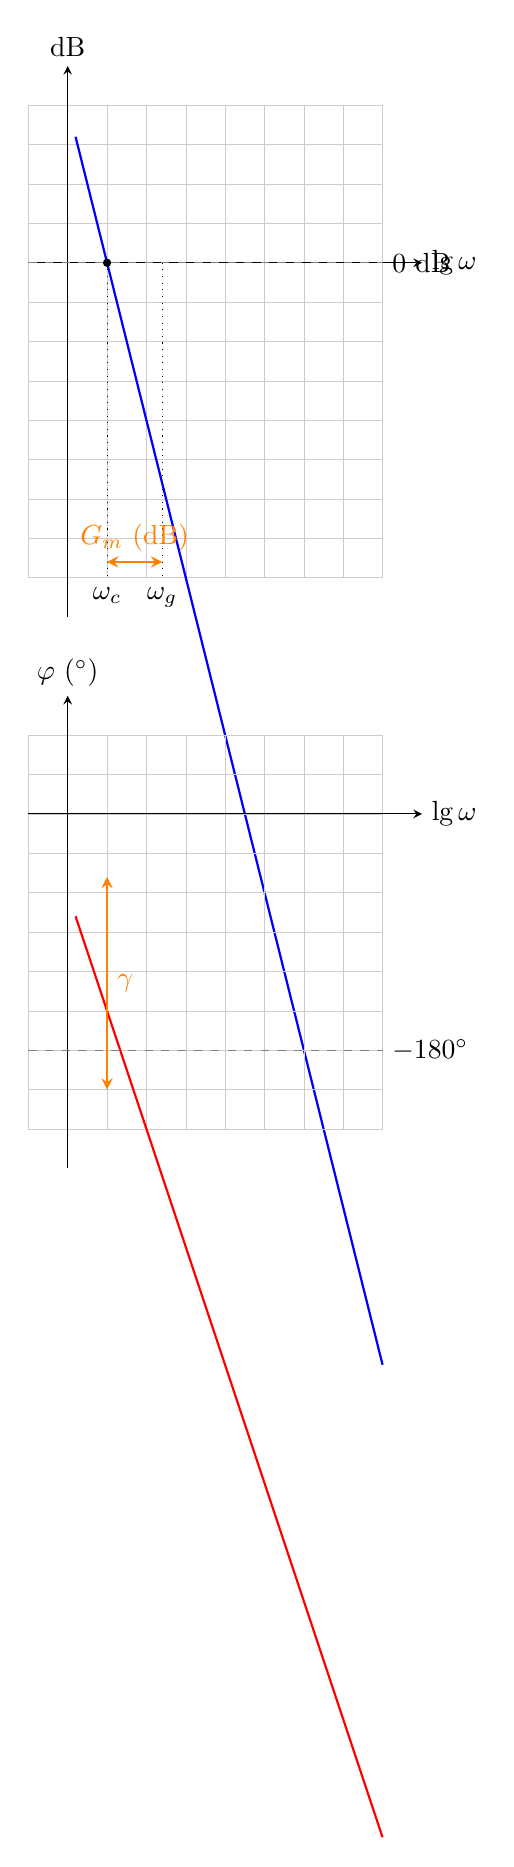
\begin{tikzpicture}[
    ctrlMarginGridStyle/.style={gray!40, very thin},
    ctrlMarginMagStyle/.style={blue, thick},
    ctrlMarginPhaseStyle/.style={red, thick},
    ctrlMarginArrowStyle/.style={<->, thick, orange},
    >=stealth
]
    % --- Bode 图 ---
    % 幅频
    \begin{scope}
        \draw[ctrlMarginGridStyle] (-0.5,-4) grid[step=0.5] (4,2);
        \draw[->] (-0.5,0) -- (4.5,0) node[right] {$\lg\omega$};
        \draw[->] (0,-4.5) -- (0,2.5) node[above] {dB};

        \draw[ctrlMarginMagStyle, domain=0.1:4, samples=100, smooth]
            plot (\x, {2-4*\x});

        % 0dB 线
        \draw[dashed, gray] (-0.5,0) -- (4,0) node[right, black] {$0$ dB};

        % 标注 omega_c
        \draw[dotted] (0.5,0) -- (0.5,-4);
        \node[below] at (0.5,-4) {$\omega_c$};
        \fill (0.5,0) circle (1.5pt);

        % 标注 omega_g
        \draw[dotted] (1.2,0) -- (1.2,-4);
        \node[below] at (1.2,-4) {$\omega_g$};

        \draw[ctrlMarginArrowStyle] (0.5,-3.8) -- (1.2,-3.8)
            node[midway, above] {$G_m$ (dB)};
    \end{scope}

    % 相频
    \begin{scope}[yshift=-7cm]
        \draw[ctrlMarginGridStyle] (-0.5,-4) grid[step=0.5] (4,1);
        \draw[->] (-0.5,0) -- (4.5,0) node[right] {$\lg\omega$};
        \draw[->] (0,-4.5) -- (0,1.5) node[above] {$\varphi$ ($^{\circ}$)};

        \draw[ctrlMarginPhaseStyle, domain=0.1:4, samples=100, smooth]
            plot (\x, {-1-3*\x});

        % -180 线
        \draw[dashed, gray] (-0.5,-3) -- (4,-3) node[right, black] {$-180^{\circ}$};

        % 标注
        \draw[ctrlMarginArrowStyle] (0.5,-3.5) -- (0.5,-0.8)
            node[midway, right] {$\gamma$};
    \end{scope}
\end{tikzpicture}
\caption{稳定裕度在 Bode 图上的表示}
\label{fig:stability-margins}
\end{figure}

% 第二幅 TikZ — Nyquist 图上的稳定裕度
\begin{figure}[H]
\centering
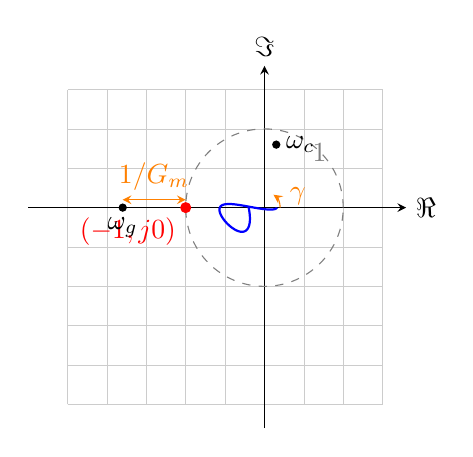
\begin{tikzpicture}[
    ctrlMarginNyqGrid/.style={gray!40, very thin},
    ctrlMarginNyqCurve/.style={blue, thick},
    ctrlMarginNyqUnitCircle/.style={dashed, gray},
    >=stealth
]
    \draw[ctrlMarginNyqGrid] (-2.5,-2.5) grid[step=0.5] (1.5,1.5);
    \draw[->] (-3,0) -- (1.8,0) node[right] {$\Re$};
    \draw[->] (0,-2.8) -- (0,1.8) node[above] {$\Im$};

    % 单位圆
    \draw[ctrlMarginNyqUnitCircle] (0,0) circle (1);
    \node[gray] at (0.7,0.7) {1};

    % (-1, j0)
    \fill[red] (-1,0) circle (2pt);
    \node[red, below left] at (-1,0) {$(-1,j0)$};

    % Nyquist 曲线示意
    \draw[ctrlMarginNyqCurve,
        domain=0:6.28, samples=100, smooth,
        variable=\t]
        plot ({0.3*cos(\t r) - 0.5*exp(-0.2*\t)},
             {0.3*sin(\t r) - 0.8*exp(-0.2*\t)*sin(\t r)});

    % 与单位圆交点
    \fill (0.15, 0.8) circle (1.5pt);
    \node[right] at (0.15, 0.8) {$\omega_c$};

    % 相位裕度角
    \draw[orange, ->] (0.2, 0) arc (0:55:0.2);
    \node[orange, right] at (0.2, 0.15) {$\gamma$};

    % 与负实轴交点
    \fill (-1.8, 0) circle (1.5pt);
    \node[below] at (-1.8, 0) {$\omega_g$};
    \draw[<->, orange] (-1.8, 0.1) -- (-1, 0.1)
        node[midway, above] {$1/G_m$};
\end{tikzpicture}
\caption{稳定裕度在 Nyquist 图上的表示}
\label{fig:margins-nyquist}
\end{figure}

% ============================================================
\section{闭环频率特性}
% ============================================================

\subsection{闭环频域指标}

对于单位反馈系统，闭环传递函数为
\[
\Phi(s) = \frac{G(s)}{1 + G(s)}
\]
闭环频率特性 $\Phi(j\omega)$ 的特征量为：

\begin{mydefinition}{闭环频域指标}
\begin{enumerate}
    \item \textbf{谐振峰值 $M_p$}：闭环幅频特性的最大值：
    \[
    M_p = \max_{\omega} |\Phi(j\omega)|
    \]
    \item \textbf{谐振频率 $\omega_r$}：达到 $M_p$ 时所对应的频率。
    \item \textbf{带宽频率 $\omega_b$}：闭环幅频特性降到 $0.707|\Phi(j0)|$（即 $-3$ dB）时的频率。
    \item \textbf{剪切频率 $\omega_c$}：$|\Phi(j\omega_c)| = 1$ 时的频率。
\end{enumerate}
\end{mydefinition}

带宽 $\omega_b$ 是表征系统响应速度的重要指标：带宽越大，系统响应越快，但抗高频噪声能力越弱。

\subsection{Nichols 图}

Nichols 图是以开环相频 $\angle G(j\omega)$ 为横坐标、开环对数幅频 $20\lg|G(j\omega)|$ 为纵坐标、$\omega$ 为参变量的图。在 Nichols 图上附加\textbf{等 M 圆}（等闭环幅值线）和\textbf{等 N 圆}（等闭环相位线）后，可以直接从开环特性读出闭环特性。

\begin{myformula}
\left|\frac{G(j\omega)}{1+G(j\omega)}\right| = M \quad\Rightarrow\quad
\left|\frac{G}{1+G}\right|^2 = \frac{x^2 + y^2}{(1+x)^2 + y^2} = M^2
\end{myformula}

其中 $G(j\omega) = x + jy$。整理得到等 M 圆方程：
\[
\left(x + \frac{M^2}{M^2 - 1}\right)^2 + y^2 = \left(\frac{M}{M^2 - 1}\right)^2
\]

\begin{remark}
Nichols 图是频域设计的重要工具。设计者可以在 Nichols 图上直观地看到开环频率特性形状与闭环性能指标（$M_p$、$\omega_b$）之间的关系，从而指导控制器的设计。
\end{remark}

% --- Nichols 图 TikZ ---
\begin{figure}[H]
\centering
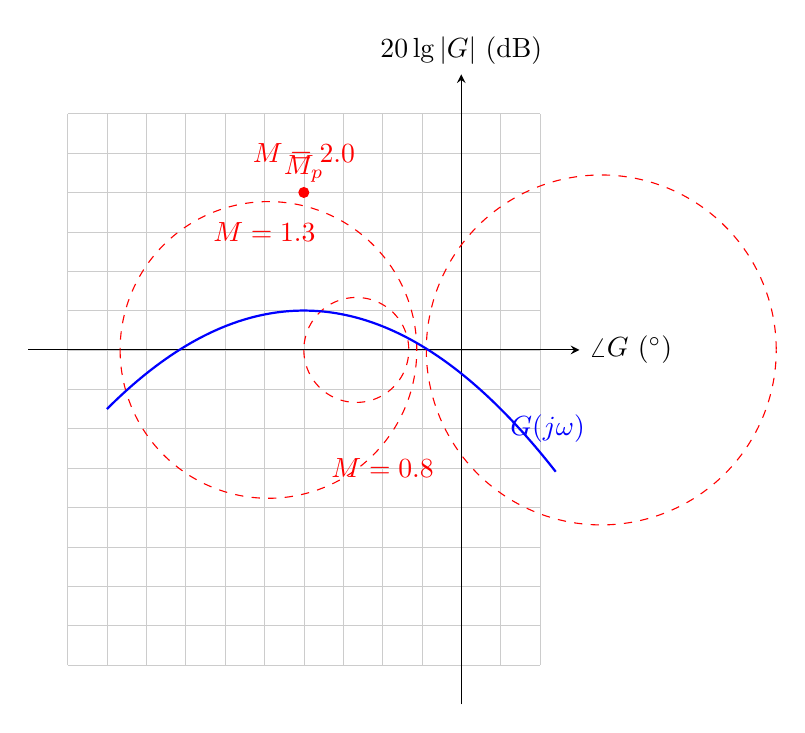
\begin{tikzpicture}[
    ctrlNicholsGridStyle/.style={gray!40, very thin},
    ctrlNicholsCurveStyle/.style={blue, thick},
    ctrlNicholsMCircle/.style={red, dashed},
    >=stealth
]
    % 坐标设置
    \draw[ctrlNicholsGridStyle] (-5,-4) grid[step=0.5] (1,3);
    \draw[->] (-5.5,0) -- (1.5,0) node[right] {$\angle G$ ($^{\circ}$)};
    \draw[->] (0,-4.5) -- (0,3.5) node[above] {$20\lg|G|$ (dB)};

    % 0dB 线
    \draw[dashed] (-5,0) -- (1,0);

    % 等 M 圆示例（M=1.3, M=2.0, M=0.8）
    \foreach \M in {0.8, 1.3, 2.0} {
        \draw[ctrlNicholsMCircle, domain=-3.14:3.14, samples=100, smooth,
            variable=\t]
            plot ({-(\M*\M)/(\M*\M-1) + (\M/(\M*\M-1))*cos(\t r)},
                 {(\M/(\M*\M-1))*sin(\t r)});
    }

    % 示例开环曲线
    \draw[ctrlNicholsCurveStyle,
        domain=-4.5:1.2, samples=80, smooth]
        plot (\x, {0.5 - 0.2*(\x+2)*(\x+2)});

    % 标注
    \node[red] at (-2.5, 1.5) {$M=1.3$};
    \node[red] at (-2, 2.5) {$M=2.0$};
    \node[red] at (-1, -1.5) {$M=0.8$};
    \node[blue, right] at (0.5, -1) {$G(j\omega)$};

    % 谐振点
    \fill[red] (-2, 2) circle (2pt);
    \node[red, above] at (-2, 2) {$M_p$};
\end{tikzpicture}
\caption{Nichols 图与等 M 圆}
\label{fig:nichols}
\end{figure}

% ============================================================
\section{频域特性与时域指标的关系}
% ============================================================

对于典型的二阶系统，频域指标与时域指标之间存在简洁的解析关系。

\subsection{二阶系统的频域-时域关系}

设二阶系统 $\Phi(s) = \frac{\omega_n^2}{s^2 + 2\zeta\omega_n s + \omega_n^2}$，$0 < \zeta < 1$。

\begin{myformula}
M_p = \frac{1}{2\zeta\sqrt{1-\zeta^2}},\quad
\omega_r = \omega_n\sqrt{1-2\zeta^2}\quad (\zeta \leq 0.707)
\end{myformula}

\begin{myformula}
\omega_b = \omega_n\sqrt{1-2\zeta^2 + \sqrt{2 - 4\zeta^2 + 4\zeta^4}}
\end{myformula}

\[
\omega_c \approx \omega_n\sqrt{\sqrt{1+4\zeta^4} - 2\zeta^2}
\]

时域指标（超调量 $\sigma\%$，调节时间 $t_s$）与频域指标的关系：

\begin{myTheorem}{频域-时域关系公式}
对于二阶系统，频域指标与时域指标满足近似关系：
\begin{align}
    \sigma\% &\approx 0.16 + 0.4(M_p - 1),\quad 1 \leq M_p \leq 1.8 \\
    t_s &\approx \frac{k\pi}{\omega_c},\quad k = 2\sim 3
\end{align}
更精确的关系为：
\[
t_s \omega_c \approx \frac{4}{\zeta}\sqrt{\sqrt{1+4\zeta^4} - 2\zeta^2}
\]
\end{myTheorem}

\begin{remark}
对于高阶系统，可以用{\heiti 主导极点}概念近似为二阶系统进行分析。通常要求主导极点与其他极点实部之比大于5，且不存在靠近虚轴的零点。
\end{remark}

\subsection{由频域指标设计系统}

基于频域指标的设计方法可归纳为：
\begin{enumerate}
    \item 根据稳态精度要求确定开环增益 $K$。
    \item 根据期望的 $\omega_c$ 和 $\gamma$ 设计中频段形状。
    \item 高频段尽可能陡峭以抑制噪声。
    \item 低频段斜率反映无差度，斜率为 $-20\nu$ dB/dec。
\end{enumerate}

\begin{example}
某单位反馈系统要求：速度误差系数 $K_v = 20$，相位裕度 $\gamma \geq 50^{\circ}$，截止频率 $\omega_c \geq 2$ rad/s。试确定满足要求的开环传递函数形式。

解：由 $K_v=20$ 可知系统至少含一个积分环节，且 $K=20$。设
\[
G(s) = \frac{20}{s}\cdot\frac{1}{Ts+1}
\]
在 $\omega=2$ 处，$|G(j2)| = 20/(2\sqrt{1+4T^2})$，令其等于 1 解得 $T$。由 $\gamma = 90^{\circ} - \arctan(2T) \geq 50^{\circ}$ 可得 $T \leq 0.42$。取 $T=0.4$，则 $G(s) = 20/[s(0.4s+1)]$ 满足要求。
\end{example}

% ============================================================
\section{Python 频域分析仿真}
% ============================================================

以下 Python 代码演示了如何利用 control 库进行频域分析，包括绘制 Bode 图、Nyquist 图和计算稳定裕度。

\begin{lstlisting}[language=Python]
import numpy as np
import matplotlib.pyplot as plt
try:
    import control as ct
except ImportError:
    print("请安装 control 库: pip install control")
    exit(1)

# 定义开环传递函数 G(s) = 20 / [s(s+1)(s+2)]
num = [20]
den = [1, 3, 2, 0]  # s(s+1)(s+2) = s^3 + 3s^2 + 2s
G = ct.TransferFunction(num, den)

# 计算稳定裕度
gm, pm, wg, wp = ct.margin(G)
print(f"幅值裕度 Gm = {gm:.3f} ({20*np.log10(gm):.2f} dB)")
print(f"相位裕度 Pm = {pm:.2f} 度")
print(f"相位穿越频率 wg = {wg:.3f} rad/s")
print(f"幅值穿越频率 wc = {wp:.3f} rad/s")

# 绘制 Bode 图
plt.figure(figsize=(10, 8))
ct.bode_plot(G, dB=True, Hz=False, grid=True)
plt.suptitle("Bode 图", fontsize=14)
plt.tight_layout()
plt.show()

# 绘制 Nyquist 图
plt.figure(figsize=(8, 8))
ct.nyquist_plot(G, omega=np.logspace(-2, 2, 500))
plt.title("Nyquist 图")
plt.grid(True)
plt.show()

# 闭环频率特性
T = ct.feedback(G, 1)
plt.figure(figsize=(8, 4))
mag, phase, omega = ct.bode(T, dB=True, Hz=False, plot=False)
plt.subplot(1, 2, 1)
plt.semilogx(omega, 20*np.log10(mag))
plt.grid(True)
plt.xlabel("频率 (rad/s)")
plt.ylabel("幅值 (dB)")
plt.title("闭环幅频特性")

# 求取闭环指标
mag_linear = mag
Mp = np.max(mag_linear)
omega_r = omega[np.argmax(mag_linear)]
# 带宽：幅值降到 0.707 倍零频值
dc_gain = mag_linear[0]
idx_bw = np.where(mag_linear < 0.707 * dc_gain)[0]
omega_b = omega[idx_bw[0]] if len(idx_bw) > 0 else omega[-1]
print(f"谐振峰值 Mp = {Mp:.3f}")
print(f"谐振频率 wr = {omega_r:.3f} rad/s")
print(f"带宽频率 wb = {omega_b:.3f} rad/s")

plt.show()
\end{lstlisting}

% ============================================================
\section{本章小结}
% ============================================================

本章系统介绍了频域分析的基本理论和方法。频率特性是联系系统传递函数与动态性能的桥梁。Bode 图因其叠加性和渐近线绘制方法而成为工程上最常用的工具；Nyquist 稳定判据从复变函数论出发，给出了严格的闭环稳定性条件。稳定裕度概念将稳定性从"是/否"的二值判断扩展到"好/坏"的定量度量，为系统校正提供了依据。闭环频域指标 $M_p$、$\omega_r$、$\omega_b$ 与时域指标之间存在定量关系，使得频域设计结果可以直接预测时域响应品质。

在下一章中，我们将利用频域分析工具进行系统校正设计，通过引入补偿器改善系统的稳态和动态性能。
